\documentclass{article} % For LaTeX2e
\usepackage{nips14submit_e,times}
\usepackage{amsmath}
\usepackage{amsthm}
\usepackage{amssymb}
\usepackage{mathtools}
\usepackage{hyperref}
\usepackage{url}
\usepackage{algorithm}
\usepackage[noend]{algpseudocode}
%\documentstyle[nips14submit_09,times,art10]{article} % For LaTeX 2.09

\usepackage{mathrsfs}
\usepackage{graphicx}
\usepackage{caption}
\usepackage{subcaption}

\def\eQb#1\eQe{\begin{eqnarray*}#1\end{eqnarray*}}
\def\aB#1\aE{\begin{align*}#1\end{align*}}
\def\eQnb#1\eQne{\begin{align}#1\end{align}}
\providecommand{\e}[1]{\ensuremath{\times 10^{#1}}}
\providecommand{\pb}[0]{\pagebreak}

\newcommand{\E}{\mathrm{E}}
\newcommand{\Var}{\mathrm{Var}}
\newcommand{\Cov}{\mathrm{Cov}}

\def\Qb#1\Qe{\begin{question}#1\end{question}}
\def\Sb#1\Se{\begin{solution}#1\end{solution}}

\usepackage{scalerel,stackengine}
\stackMath
\newcommand\reallywidehat[1]{%
\savestack{\tmpbox}{\stretchto{%
  \scaleto{%
    \scalerel*[\widthof{\ensuremath{#1}}]{\kern-.6pt\bigwedge\kern-.6pt}%
    {\rule[-\textheight/2]{1ex}{\textheight}}%WIDTH-LIMITED BIG WEDGE
  }{\textheight}% 
}{0.5ex}}%
\stackon[1pt]{#1}{\tmpbox}%
}

\newenvironment{claim}[1]{\par\noindent\underline{Claim:}\space#1}{}
\newtheoremstyle{quest}{\topsep}{\topsep}{}{}{\bfseries}{}{ }{\thmname{#1}\thmnote{ #3}.}
\theoremstyle{quest}
\newtheorem*{definition}{Definition}
\newtheorem*{theorem}{Theorem}
\newtheorem*{lemma}{Lemma}
\newtheorem*{question}{Question}
\newtheorem*{preposition}{Preposition}
\newtheorem*{exercise}{Exercise}
\newtheorem*{challengeproblem}{Challenge Problem}
\newtheorem*{solution}{Solution}
\newtheorem*{remark}{Remark}
\usepackage{verbatimbox}
\usepackage{listings}
\title{Harmonic Analysis:  \\
Final Exam}


\author{
Youngduck Choi \\
CIMS \\
New York University\\
\texttt{yc1104@nyu.edu} \\
}


% The \author macro works with any number of authors. There are two commands
% used to separate the names and addresses of multiple authors: \And and \AND.
%
% Using \And between authors leaves it to \LaTeX{} to determine where to break
% the lines. Using \AND forces a linebreak at that point. So, if \LaTeX{}
% puts 3 of 4 authors names on the first line, and the last on the second
% line, try using \AND instead of \And before the third author name.

\newcommand{\fix}{\marginpar{FIX}}
\newcommand{\new}{\marginpar{NEW}}

\nipsfinalcopy % Uncomment for camera-ready version

\begin{document}


\maketitle

\begin{abstract}
This work contains a solution to the Final Exam
of Harmonic Analysis 2016 at Courant Institute of Mathematical Sciences.
\end{abstract}

\bigskip

\begin{question}[1]
\hfill
\begin{figure}[h!]
  \centering
    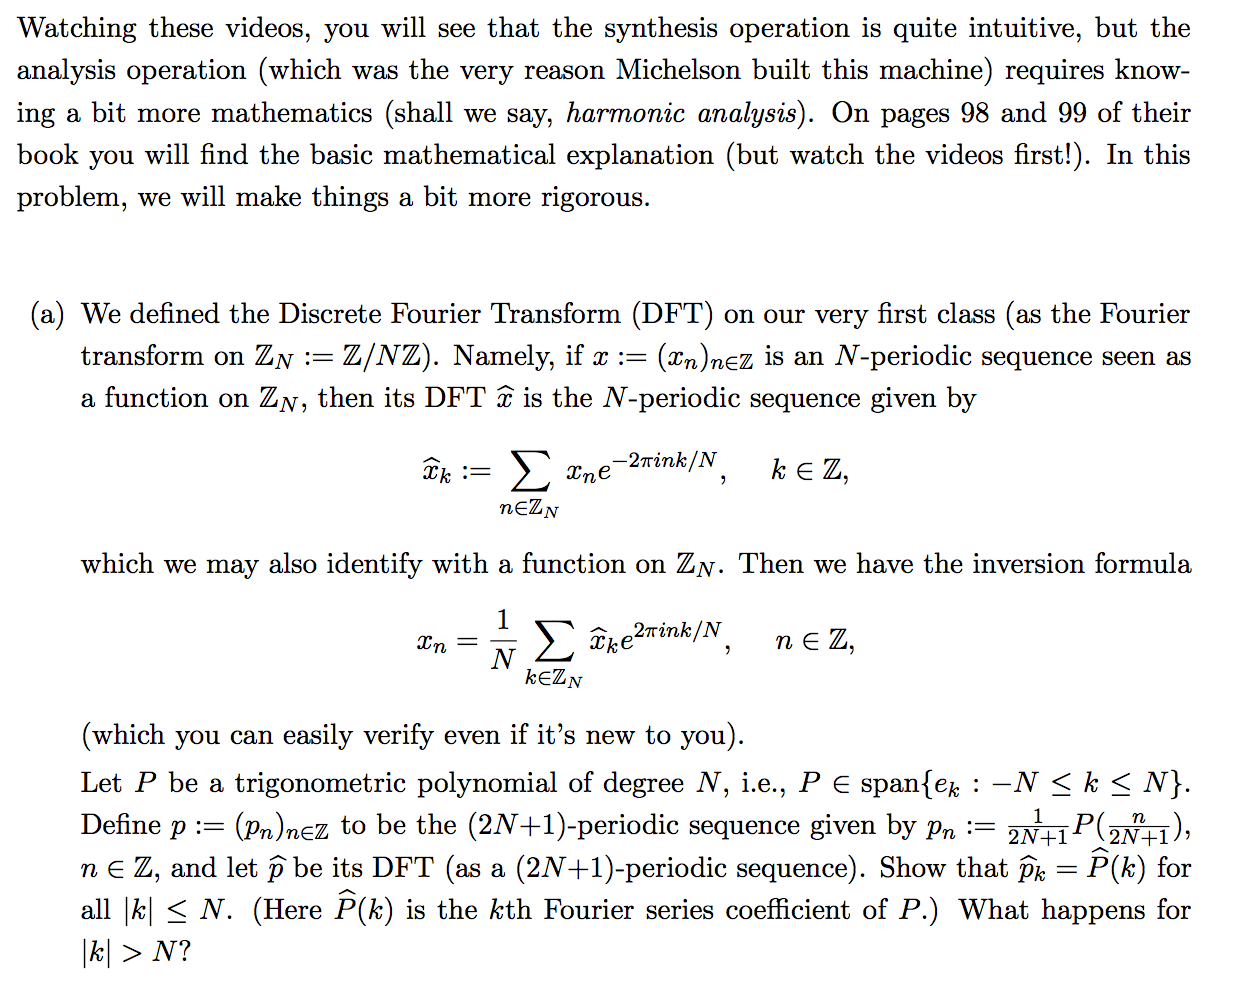
\includegraphics[width=0.8\textwidth]{HA-f-1.png}
\end{figure}
\end{question}

\newpage 

\begin{solution} \hfill \\
\textbf{(a)} Let $P$ be a trig polynomial defined on $\mathbb{T}$ of degree $N$, i.e. 
\eQb
P &=& \sum_{|k| \leq N} a_k e_k,
\eQe 
where $a_k$s are the complex coefficients. 
Suppose $|k| \leq N$. We trivially know that $\hat{P}(k) = a_k$. We compute
\eQb
\widehat{p_k} &=& \sum_{n \in \mathbb{Z}_{2N+1}} p_n e^{\frac{-2\pi i n k}{2N+1}} 
= \sum_{n \in \mathbb{Z}_{2N+1}} \dfrac{1}{2N+1} P(\dfrac{n}{2N + 1}) e^{-\frac{2\pi i n k}{2N+1}} \\
&=& \dfrac{1}{2N+1}\sum_{n \in \mathbb{Z}_{2N+1}} \left( 
\sum_{|l| \leq N} a_l e_{l}(\dfrac{n}{2N+1}) \right) 
e^{-\frac{2\pi i n k}{2N+1}}  
= \dfrac{1}{2N+1}\sum_{n \in \mathbb{Z}_{2N+1}} \left( 
\sum_{|l| \leq N} a_l e^{\frac{2\pi i l n}{2N+1}} \right) 
e^{-\frac{2\pi i n k}{2N+1}} \\
&=& \dfrac{1}{2N+1}\sum_{n \in \mathbb{Z}_{2N+1}} \left( 
\sum_{|l| \leq N} a_l e^{\frac{2\pi i (l-k) n}{2N+1}} \right) 
= \dfrac{1}{2N+1} \sum_{|l| \leq N} \left( a_l \sum_{n \in \mathbb{Z}_{2N+1}} e^{\frac{2\pi i (l-k)n}{2N+1}}
\right) \\
&=& \dfrac{1}{2N+1} \sum_{|l| \leq N; l \neq k} \left( 
a_l \sum_{n \in \mathbb{Z}_{2N+1}} e^{\frac{2\pi i (l-k)n}{2N+1}} 
\right)
+ \dfrac{1}{2N+1} \sum_{|l| \leq N; l = k} \left( 
a_l \sum_{n \in \mathbb{Z}_{2N+1}} e^{\frac{2\pi i (l-k)n}{2N+1}} \right) \\
&=& 0 + \dfrac{1}{2N+1}(2N+1) a_k = a_k,
\eQe
as the sum of any $N$-th root of unity is zero, thereby forcing the first term of the second last equation 
to be $0$. 
For $|k| > N$, we trivially see that $\widehat{p}_k = 0$, and $\hat{P}(k) = 0$ as well.
\hfill $\qed$
\end{solution}

\bigskip

\begin{question}[1-2]
\hfill
\begin{figure}[h!]
  \centering
    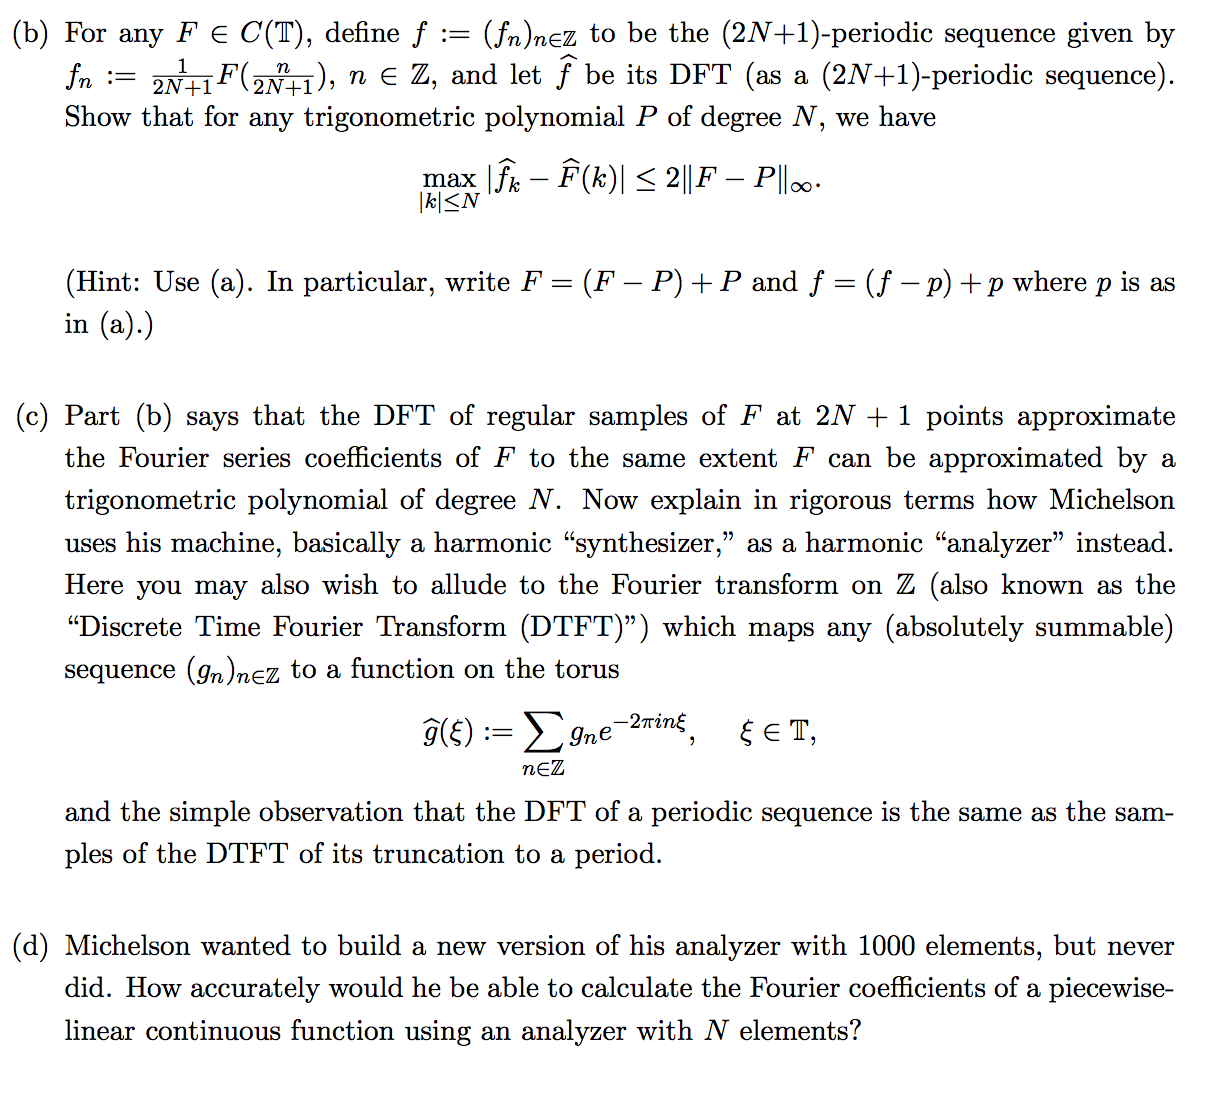
\includegraphics[width=0.8\textwidth]{HA-f-1-2.png}
\end{figure}
\end{question}
\begin{solution} \hfill \\
\textbf{(b)} Let $ f \in C(\mathbb{T})$, and $P$ be a trig polynomial of degree $N$. 
Define as before $f \triangleq (f_n)_{n \in \mathbb{Z}}$ to be the $(2N+1)$-periodic sequence given by 
\eQb
f_n \triangleq \dfrac{1}{2N+1}F(\dfrac{n}{2N+1}).
\eQe
With $F = (F- P) + P$ and $f = (f-p) + p$, by the result of $(a)$, for any $|k| \leq N$, we see that
\eQb \label{eq1}
|\widehat{f_k} - \hat{F}_k| &=& |\reallywidehat{\{(f-p) + p\}}_k - 
\reallywidehat{(F-P)+P}(k)| 
= |\widehat{(f-p)}_k - \reallywidehat{(F-P)}(k) + \hat{p}_k - \hat{P}(k)| \nonumber \\
&\leq&  
|\widehat{(f-p)}_k| + |\reallywidehat{(F-P)}(k)| + | \hat{p}_k - \hat{P}(k)| 
=
|\widehat{(f-p)}_k| + |\reallywidehat{(F-P)}(k)|. \>\> (1)
\eQe
Now, in view of \eqref{eq1}, and the fact that $N$ is finite, it suffices to show that for any $|k| \leq N$,
\eQb
|\widehat{(f-p)}_k| \leq ||F-P||_{\infty} \> \text{and} \> |\reallywidehat{(F-P)}(k)| \leq ||F-P||_{\infty}.
\eQe
Now, for $|k| \leq N$, the first inequality follows, as
\eQb
|\widehat{(f-p)}_k| &=& |\sum_{n \in \mathbb{Z}_{2N+1}} (f-p)_{n} e^{\frac{-2\pi i n k}{2N+1}}| \\
&=& |\dfrac{1}{2N+1} \sum_{n \in \mathbb{Z}_{2N+1}} (F(\dfrac{n}{2N+1}) - P(\dfrac{n}{2N+1}) )
e^{\frac{-2\pi i n k}{2N+1}}| \\
&\leq& \dfrac{1}{2N+1} \sum_{n \in \mathbb{Z}_{2N+1}} |F(\dfrac{n}{2N+1}) - P(\dfrac{n}{2N+1})| = ||F-P||_{\infty}.  
\eQe

Likewise, for $|k| \leq N$, the second inequality, as $F-P \in C(\mathbb{T})$, and 
\eQb
|\reallywidehat{F-P}(k)| &=& \left| \int_{\mathbb{T}} (F-P)(t)e^{-ikt} dt \right|  \leq 
\int_{\mathbb{T}} |(F-P)(t)| dt \\
&=& ||F-P||_{1} \leq ||F-P||_{\infty}.
\eQe
Therefore, we have that for any trig polynomial of degree $N$, $P$, 
\eQb
\max_{|k| \leq N} | \hat{f}_{k} - \hat{F}(k)| &\leq& 2||F- P||_{\infty},
\eQe
as required. 

\bigskip

\textbf{(c)}

\bigskip

\textbf{(d)}


\end{solution}

\newpage

\begin{question}[2]
\hfill
\begin{figure}[h!]
  \centering
    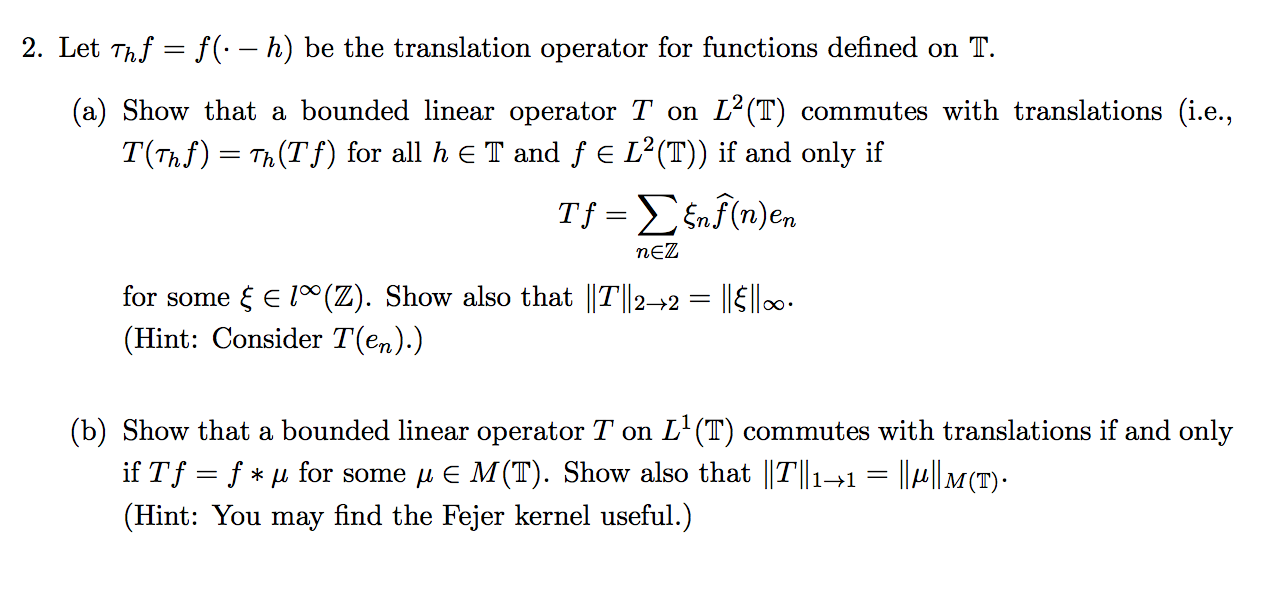
\includegraphics[width=0.8\textwidth]{HA-f-2.png}
\end{figure}
\end{question}
\begin{solution} \hfill \\
\textbf{(a)}
We first prove the equivalence for $\{e_n\}$. 
Fix $ h \in \mathbb{T}$.
Suppose that, for some $\xi \in l^{\infty}(\mathbb{Z})$, we have
\eQb
Te_n &=& \sum_{n \in \mathbb{Z}} \xi_{n} \hat{f}(n) e_n, 
\eQe
for all $n$. As $\hat{e_n}(k) = 1$, if $k = n$ and $0$ otherwise, it follows that, for all $n$,
\eQb
Te_n &=& \xi_{n} e_n,
\eQe
and, by linearity of $T$,
\eQb
T(\tau_{h}(e_n)) &=& T(e^{2\pi i n(\cdot-h)}) = e^{2\pi i n h} T(e_n) 
= e^{-2\pi i n h} \xi_n e_n = \tau_h(T(e_n)).
\eQe
Conversely, assume that $T(\tau_h e_n) = T($.

As $Te_n \in L^2$, by Riemann-Lebesgue lemma, it follows that
\eQb
\xi_n = \widehat{Te_n}(n) \to 0,
\eQe 
as $n \to \infty$, so $\{ \xi_n \} \in l^{\infty}(\mathbb{Z})$, as required.

\smallskip

Now, we argue that the equivalence can be extended to any $f \in L^2$. Suppose that the operator
commutes with the translation operator for any $e_n$. Then, it follows that, for any $f \in L^2$,
\eQb
T(\tau_h f) &=& T(\tau_h \sum_{n \in \mathbb{Z}} \hat{f}(n)e_n) = \sum_{n \in \mathbb{Z}} \hat{f}(n)
T(\tau_h e_n) \\
&=& \sum_{n \in \mathbb{Z}} \hat{f}(n) \tau_h(Te_n) = \tau_h(T f). 
\eQe
The converse holds trivially. Now, suppose that the operator has the given description with respect to
$\{e_n\}$. It follows that, for any $f \in L^2$,
\eQb
Tf &=& T(\sum_{n \in \mathbb{Z}} \hat{f}(n) e_n ) = \sum_{n \in \mathbb{Z}} \hat{f}(n) T(e_n) = 
\sum_{n \in \mathbb{Z}} \xi_n \hat{f}(n)  e_n. 
\eQe
The converse in this case also holds trivially. Thus, we have shown the desired equivalence. 

\smallskip

We now argue that $||T||_{2 \to 2} = ||\xi||_{\infty}$. By Parseval, we obtain
\eQb
||T||_{2 \to 2} &=& \sup_{||f||_{2} = 1} ||Tf||_{2} = \sup_{||f||_{2} =1} 
(\sum_{n \in \mathbb{Z}} |\xi_n \hat{f}(n)|^2)^{\frac{1}{2}}  \\ &\leq& \sup_{||f||_{2} = 1} 
||\xi||_{\infty} (\sum_{n \in \mathbb{Z}}|\hat{f}(n)|^2 )^{\frac{1}{2}} = ||\xi||_{\infty}. 
\eQe 
Now, we construct $f \in L^2$, such that $||Tf|| = ||\xi||_{\infty}$.

\bigskip

\textbf{(b)} Consider the Fejer kernel, denoted by $\{ K_n \}$. 
Firstly, observe that as the Fejer kernel is an approximate identity,
we have $\sup_{N} \int_{0}^{1} |K_n(x)|dx < \infty$, so 
we can extract a subsequence $\{ K_{n_l} \}$ 
such that $K_{n_l} \to \mu$ weakly in $L^1$, for some $\mu \in M(\mathbb{T})$.
 For notational convenience, we
relabel the subsequence as $\{ K_n \}$. Now, assume that $T$ commutes 
with translations. It follows that, for any $f \in C(\mathbb{T})$, and $x \in \mathbb{T}$, 
\eQb
f * \mu (x) &=& \lim_{n \to \infty} \int_{\mathbb{T}} f(t)T(K_n) (x - t) dt 
= \lim_{n \to \infty} \int_{\mathbb{T}} f(t)T(K_n(x - t)) dt, \\
&=& \lim_{n \to \infty} \int_{\mathbb{T}} T(f(t)(K_n) (x - t)) dt, 
= \lim_{n \to \infty} T\left(\int_{\mathbb{T}} f(t) K_n(x-t) dt \right),
\eQe
which via boundedness of $T$ and the fact that $f \in C(\mathbb{T})$, 
\eQb
\lim_{n \to \infty} (f*K_n) (x) = f(x),
\eQe
implies that
\eQb
f* \mu(x)&=& T \left( \lim_{n \to \infty} \int_{\mathbb{T}} f(t) K_n(x-t) dt \right) = Tf(x),
\eQe  
as required. Now, as $C(\mathbb{T})$ is dense in $L^1(\mathbb{T})$, it follows that
\eQb
f* \mu &=& Tf 
\eQe 


\end{solution}

\newpage

\begin{question}[3]
\hfill
\begin{figure}[h!]
  \centering
    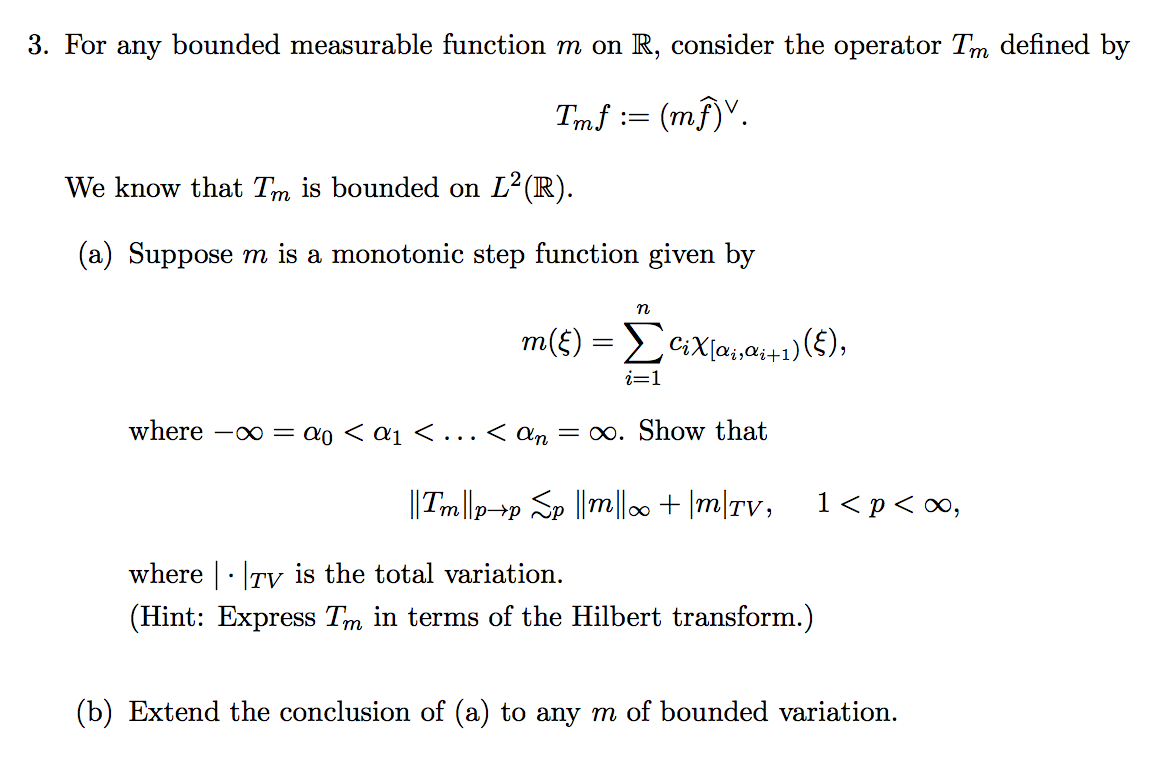
\includegraphics[width=0.8\textwidth]{HA-f-3.png}
\end{figure}
\end{question}
\begin{solution} \hfill \\
\textbf{(a)} We fix the index in the definition of $m$ to start at $0$ and end at $n-1$.
 Suppose $m$ is a monotonic step function given by 
\eQb
m &=& \sum_{i=0}^{n-1} c_i X_{[\alpha_{i}, \alpha_{i+1})}.
\eQe
As $T_{[0,\infty)} = (iH + \dfrac{1}{2}I)$ (this fact was discussed in class), we have that
\eQb
T_{[a,\infty)}f &=& e^{2\pi i a x} iHf(x) + \dfrac{1}{2} f(x),
\eQe
so
\eQb
T_{m}f &=& T_{\sum_{i=0}^{n-1} c_i X_{[\alpha_i, \alpha_{i+1}]}} 
= c_0 I + \sum_{i=0}^{n-2} (c_{i+1} - c_i) T_{[\alpha_{i+1},\infty)} \\
&=& c_0 I + 
 \sum_{i=0}^{n-2} (c_{i+1}-c_i)
(e^{2\pi i \alpha_{i+1}} iHf + \dfrac{1}{2}f) .
\eQe
Now, by the triangle inequality, and the fact that the Hilbert Transform is bounded on $L^p$ 
(recall that the bound constant is dependent on $p$) for 
$1 < p < \infty$, we obtain
\eQb
||T_m f||_{p} &\leq& |c_0|||f||_{p} + \sum_{i=0}^{n-2} |c_{i+1}
- c_i|(||Hf||_{p} + \dfrac{1}{2}||f||_{p}) \\
&\leq& C_p (|c_0| + \sum_{i=0}^{n-2} |c_{i+1} - c_i|) ||f||_p
\leq C_p (||m||_{\infty} + |m|_{TV}) ||f||_{p}, \\
\eQe
for some constant $C_p$, depended on $p$, so
\eQb
||T_m||_{p\to p} \leqslant_{p} (||m||_{\infty} + |m|_{TV}),
\eQe
as required.

\bigskip

\textbf{(b)}
Let $m$ be a function of bounded variation. As having a bounded variation implies being bounded, it follows that
\eQb
||m||_{\infty} < \infty. 
\eQe
Now, as $m$ is measurable,  we can 
choose a sequence of monotonic step functions that converge pointwise to $m$ such that 
$|m_n| \leq |m|$ for all $n$. Therefore, by DCT, for any $f \in L^p$, with $1 < p < \infty$,
it follows that, for the pointwise limit,
\eQb
\lim_{n \to \infty} T_{m_n} f &=& \lim_{n \to \infty} \int_{\mathbb{R}} m_n(\xi) \hat{f}(\xi)  
e^{2\pi i \xi} d\xi 
= \int_{\mathbb{R}} m(\xi)\hat{f}(\xi) e^{2\pi i \xi} d\xi = T_m f. 
\eQe
Therefore, by Fatou 
\eQb
||T_m f||_{p} \leq \liminf_{n} ||T_{m_n} f||_{p},
\eQe
and by $(a)$, and the choice of $\{m_n\}$
\eQb
||T_m f||_{p} \leq \liminf_{n} ||T_{m_n} f||_{p} \leqslant_{p} (||m||_{\infty} + |m|_{TV}),
\eQe
as required. \hfill $\qed$
\end{solution}

\bigskip

\begin{question}[4]
\hfill
\begin{figure}[h!]
  \centering
    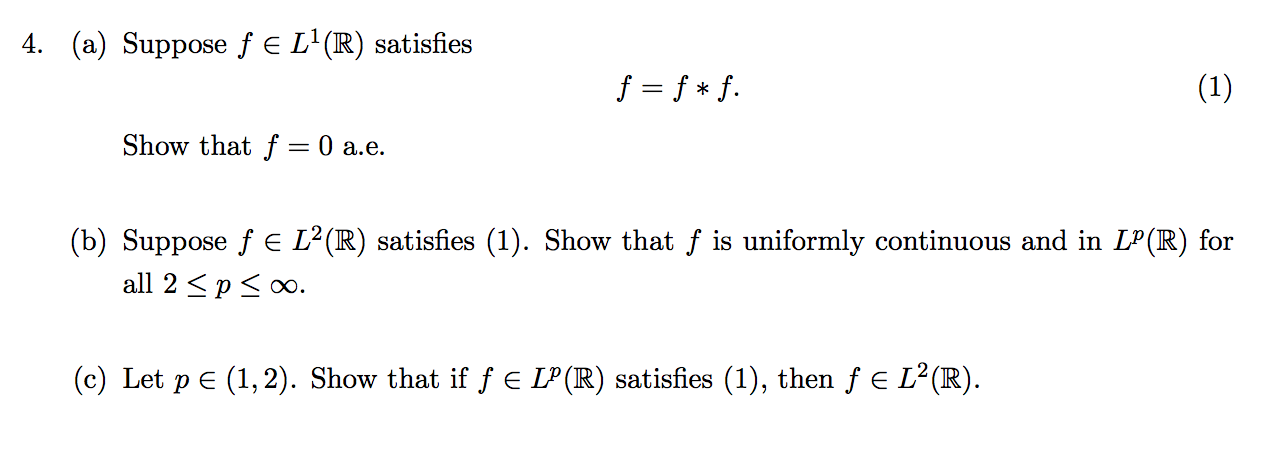
\includegraphics[width=0.8\textwidth]{HA-f-4.png}
\end{figure}
\end{question}
\begin{solution} \hfill \\

\textbf{(a)} Let $f \in L^1$. Taking the Fourier transform on both sides gives
\eQb
\hat{f} &=& \hat{f}\hat{f},
\eQe
which, with the continuity of $\hat{f}$, implies that
\eQb
\hat{f} = 0 \> \text{ a.e} \> &\text{ or }& \> \hat{f} = 1 \> \text{a.e}.
\eQe
As $\hat{f} = 1 \> \text{ a. e}$ contradicts the Riemann-Lebesgue lemma, it follows that
\eQb
\hat{f} &=& 0 \> \text{ a.e.},
\eQe
so by the inversion formula for $L^1$
\eQb
f &=& 0 \> \text{ a.e.},
\eQe 
as required.

\bigskip

\textbf{(b)} Let $f \in L^2$ such that $f = f * f$. By the same argument in the $L^1$ case, 
we have 
\eQb
\hat{f} = 0 \> \text{ a.e} \> &\text{ or }& \> \hat{f} = 1 \> \text{a.e}.
\eQe
Let $E_1 = \{ \hat{f} = 1\}$ and $E_0 = \{ \hat{f} = 0 \}$.
As $\hat{f} \in L^2$, it follows that 
\eQb
||\hat{f}||_{2} &=& (\int_{\mathbb{R}} |\hat{f}(\xi)|^2)^{\frac{1}{2}} = m(E_1)^{\frac{1}{2}} < \infty, 
\eQe
so
\eQb
m(E_1) < \infty,
\eQe
and, for any $p \geq 1$, 
\eQb
||\hat{f}||_{p} &=& (\int_{\mathbb{R}} |\hat{f}(\xi)|^p)^{\frac{1}{p}} = m(E_1)^{\frac{1}{p}} < \infty. 
\eQe
Therefore, we see that, for $1 \leq p \leq \infty$,
\eQb
\hat{f} \in L^p,
\eQe
as the infinity bound follows trivially.

\smallskip

Now, we first prove the uniform continuity of $f$. By the inversion formula for $L^2$,
we obtain
\eQb
f(x) &=& \int_{\mathbb{R}} \hat{f}(\xi)e^{2\pi i \xi x} d\xi = \int_{E_1} e^{2\pi i \xi x} d\xi. 
\eQe
Therefore, for any $\delta > 0$ and $x \in \mathbb{R}$, it follows that
\eQb
|f(x + \delta) - f(x)| &=& | \int_{E_1} e^{2\pi i \xi (x + \delta)}  - 
e^{2\pi i \xi x}| d\xi  
\leq  \int_{E_1} |e^{2\pi i \xi x }| |e^{2\pi i \xi \delta } - 1| d\xi \\
&\leq& 
\int_{E_1} |e^{2\pi i \xi \delta } - 1| d\xi. \\
\eQe
Observe that the last integral is independent of $x$, and the integrand tends to $0$,
as $\delta \to 0$. Therefore, we have shown that $f$ is uniformly continuous. 

\smallskip

We now argue that
$f \in L^p$ for $p \in [2,\infty]$. We employ Riesz-Thorin to the Fourier inversion operator. 
Since the Fourier inversion is bounded from $L^1$ to $L^{\infty}$ and from $L^2$ to $L^2$, by
Riesz-Thorin, we have that the inversion is bounded from $p$ to $q$ where $1 \leq p \leq 2$
and $q$ is the conjugate of $p$. In particular, for $2 \leq p \leq \infty$, we see that
\eQb
||f||_{p} &\leq& ||\hat{f}||_{q}, 
\eQe
where $q$ is again the conjugate of $p$.
As we have previously shown that $\hat{f} \in L^p$, for all $1 \leq p \leq \infty$, we are done.

\bigskip

\textbf{(c)} Let $f \in L^p$ such that $f = f*f$. As $p \in (1,2)$, it follows that $\hat{f} \in L^q$,
where $q$ is the conjugate of $p$.
As $\hat{f} \in L^q$, by the same argument from $(b)$, we have that $\hat{f} \in L^2$.
Therefore, we have shown that $\hat{f} \in L^2$, so $f \in L^2$, as the Fourier transform is an isometry on
$L^2$. \hfill $\qed$  

\end{solution}
\end{document}
